 \subsubsection{assign\_values\_to\_qpoints.f90}

 \subsubsection{basis\_functions\_V.f90}
 This file contains 3 functions: 
 \subsubsection{compute\_dNdx\_dNdy\_dNdz.f90}
 This subroutine computes $\partial{\bN^\upnu}/\partial x$, $\partial{\bN^\upnu}/\partial y$ and
 $\partial{\bN^\upnu}/\partial z$ at a location $r,s,t$ passed as argument.
 \subsubsection{compute\_dNdx\_dNdy.f90}
 This subroutine computes $\partial{\bN^\upnu}/\partial x$ and $\partial{\bN^\upnu}/\partial y$
 at a location $r,s$ passed as argument.
 \subsubsection{compute\_elemental\_matrices.f90}
 Improvement: only use Cmat and not Cmat2D, Cmat3D
 \subsubsection{impose\_boundary\_conditions}

 \subsubsection{template}

 \subsubsection{interpolate\_onto\_nodes.f90}

 \subsubsection{locate\_point}
 This file contains a few simple subroutines which deal with the localisation of a point 
 in the mesh. The {\tt locate\_point} subroutine receives the coordinates of a point as argument 
 and returns its reduced coordinates and the id of the element it sits in.
 It relies on 3 other subroutines ({\tt find\_ielx\_r}, {\tt find\_iely\_s}, {\tt find\_ielz\_t})
 which take as argument a coorinate (x,y,z) and return the corresponding reduced
 coordinate (r,s,t) and the integer coordinate (ielx,iely,ielz).
 \subsubsection{make\_matrix.f90}
 This subroutine loops over all elements, build their elemental matrices and rhs, 
 apply the boundary conditions ont these elemental matrices, and then 
 assembles them in the global matrix, either in CSR or in MUMPS format.
 \subsubsection{matrix\_setup\_GT.f90}

 \subsubsection{matrix\_setup\_K}

 \subsubsection{output\_mesh.f90}
 This subroutine produces the {\filenamefont meshV.vtu} file which only 
 contains the corner nodes.
 \subsubsection{output\_qpoints}

 \subsubsection{output\_solution}
 This subroutine generates the {\filenamefont solution.vtu} in the {\foldernamefont OUTPUT}
 folder. It also generates the basic ascii file {\filenamefont solution.ascii}
 \subsubsection{output\_swarm.f90}
 This subroutine produces the {\filenamefont swarm.vtu} file in the 
 {\foldernamefont OUTPUT} folder which contains the 
 swarm of particles with all their properties.
 \subsubsection{paint\_swarm}
 
 \subsubsection{postprocessors.f90}
 This subroutine computes the root mean square velocity
 and each of the average velocity components. It also 
 computes the volume using GLQ.
 \subsubsection{prescribe\_stokes\_solution.f90}
 This subroutine prescribes the velocity, pressure, temperature and strain rate components
 on the corners of each element via the {\sl analytical\_solution} subroutine.
 \subsubsection{quadrature\_setup.f90}
 This subroutine allocates all GLQ-related arrays for each element.
 It further computes the real $(x_q,y_q,z_q)$ and reduced $(r_q,s_q,t_q)$
 coordinates of the GLQ points, and assigns them their weights.
 \subsubsection{set\_default\_values}
 This subroutine assigns default values to many of the global variables.
 \subsubsection{set\_global\_parameters\_pair}

 \subsubsection{setup\_cartesian2D.f90}
 This subroutine assigns to every element the coordinates of the its velocity, pressure,
 and temperature nodes, the velocity, pressure and temperature connectivity arrays,
 the coordinates of its center (xc,yc), its integer coordinates (ielx, iely),
 and its dimensions (hx,hy).
 \subsubsection{setup\_cartesian3D.f90}
 
 \subsubsection{solve\_cg\_diagprec}
 The subroutine solves $A\cdot = b$ by means f the preconditioned Conjugate Gradient method
 and the implementation follows algorithm 2.2 on page 82 of Elman, Silvester \&
 Wathen \cite{elsw}:
 
 Choose ${\vec u}^{(0)}$, compute ${\vec \phi}^{(0)}={\bm A}\cdot {\vec u}^{(0)}$ 
 then ${\vec r}^{(0)}={\vec f}-{\vec \phi}^{(0)}$, 
 ${\vec z}^{(0)}={\bm M}^{-1}\cdot {\vec r}^{(0)}$ and set ${\vec p}^{(0)}={\vec z}^{(0)}$.
 
 For $k=0$ until convergence do
 \begin{itemize}
 \item ${\vec \phi}^{(k)}={\bm A}\cdot {\vec p}^{(k)}$
 \item compute $\alpha_k = <{\vec z}^{(k)},{\vec r}^{(k)}>/<{\vec \phi}^{(k)},{\vec p}^{(k)}>$
 \item ${\vec u}^{(k+1)}={\vec u}^{(k)}+\alpha_k {\vec p}^{(k)}$
 \item ${\vec r}^{(k+1)}={\vec r}^{(k)}-\alpha_k{\vec \phi}^{(k)}$
 \item test for convergence
 \item ${\vec z}^{(k+1)}=M^{-1} {\vec r}^{(k+1)}$
 \item $\beta_k= <{\vec z}^{(k+1)},{\vec r}^{(k+1)}>/<{\vec z}^{(k)},{\vec r}^{(k)}>$
 \item ${\vec p}^{(k+1)}={\vec z}^{(k+1)}+\beta_k {\vec p}^{(k)}$
 \end{itemize}
 The convergence test is $\| \vec{r}_{k+1} \|_2/ \| \vec{r}_{k+1} \|_2 < tol$, 
 the maximum number of iterations is set to 1000, and the relative tolerance to $tol=10^{-6}$.
 Since the preconditioned is the diagonal of the ${\bm A}$ matrix, then the inverse of 
 ${\bm M}$ is trivial to compute/apply. 
 \subsubsection{solve\_stokes}
 This subroutine solves the saddle point problem using the preconditioned 
 conjugate gradient (PCG) applied to the Schur complement $\SSS$ 
 (see Section~\ref{ss:schurpcg}).
 \subsubsection{spmv\_kernels}
 This file contains the Sparse Matrix-Vector multiplication kernels (see Section~\ref{ss:spmv}).
 \subsubsection{swarm\_setup.f90}
 This subroutine generates the swarm of particles. The layout is controled 
 by the {\tt init\_marker\_random} parameter.
 \begin{center}
 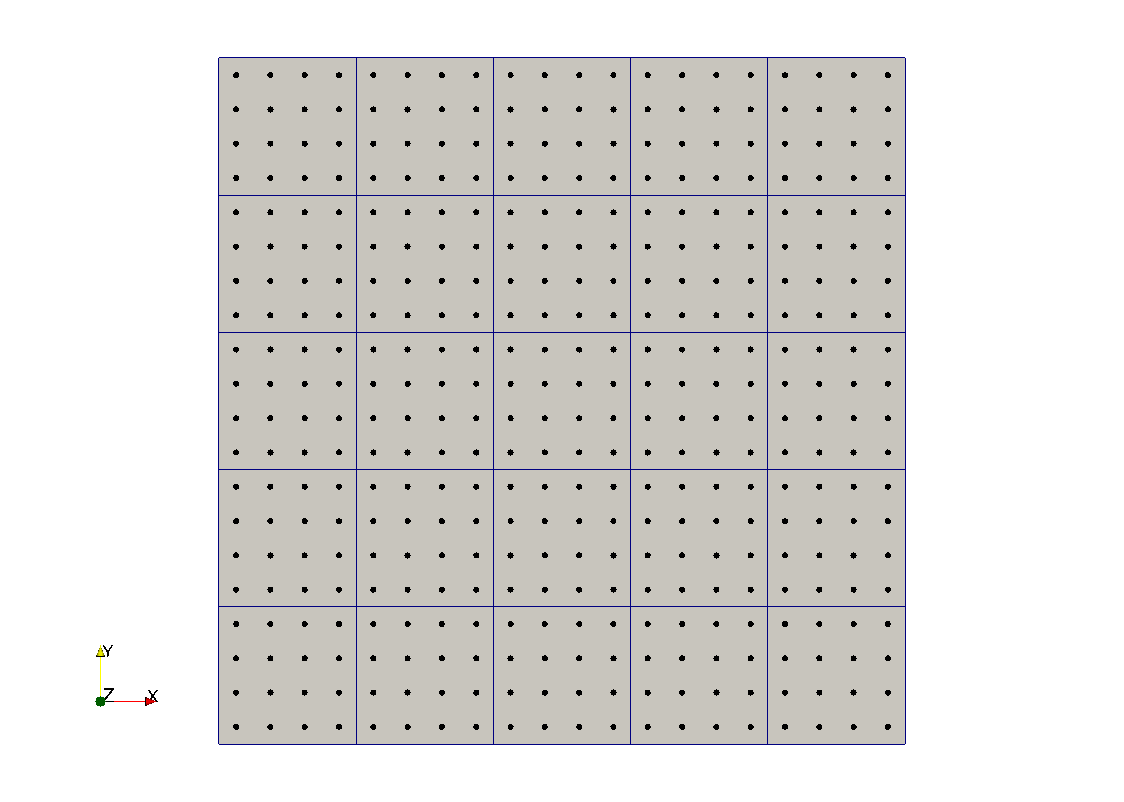
\includegraphics[width=5cm]{ELEFANT/images/swarm_reg} 
 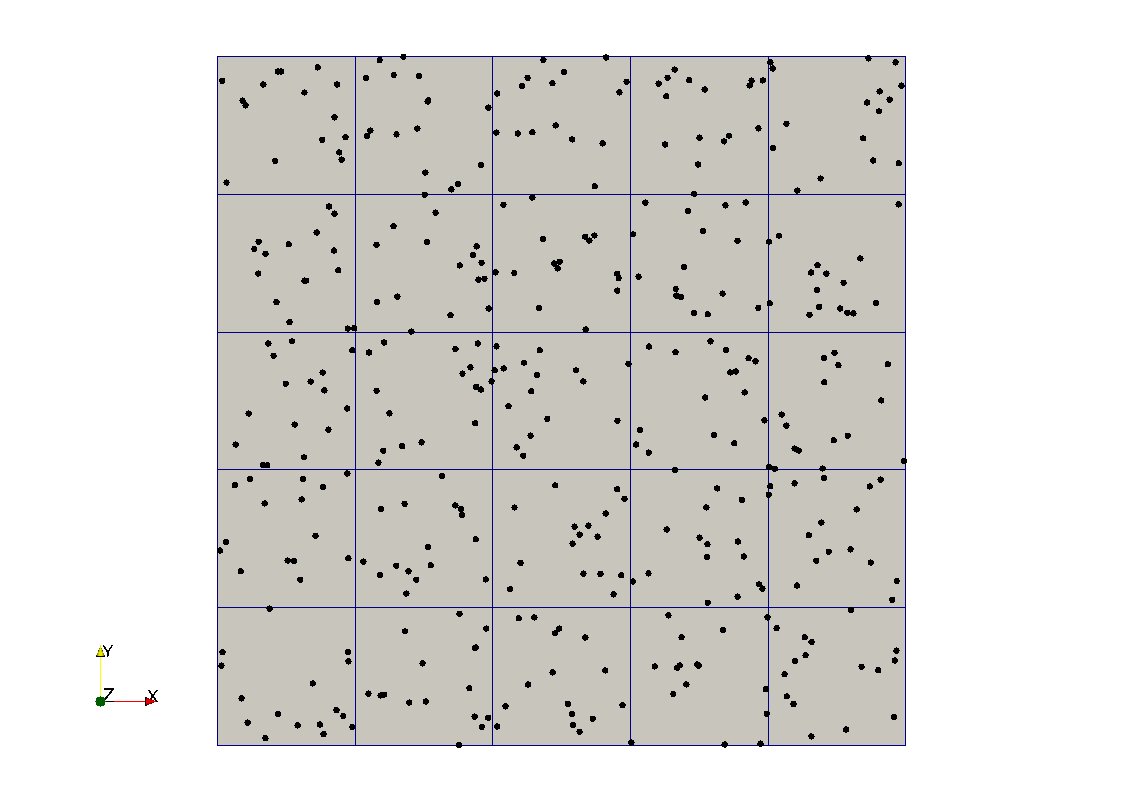
\includegraphics[width=5cm]{ELEFANT/images/swarm_rand} 
 \end{center}
 \subsubsection{template}

 \subsubsection{test\_basis\_functions}
 This subroutine tests the consistency of the basis functions. 
 An analytical velocity field is prescribed (constant, linear or quadratic) and the 
 corresponding values are computed onto the quadrature points via the 
 (derivatives of the) basis functions.
 It generates three ascii files in the {\foldernamefont OUTPUT} folder.
